\begin{problem}
{\textbf{\textsc{Ambidexterity}}}
Khi ánh sáng phân cực mặt phẳng có bước sóng \( \lambda = 500 \, \text{nm} \) đi qua một dung dịch chứa các phân tử chiral (ví dụ như glucose/DNA), ánh sáng ra khỏi dung dịch được quan sát là đã bị xoay bởi một góc \( \Delta \theta \). Trong hóa học, sự xoay quang học này được đo bằng thiết bị phân cực, và nó được sử dụng để đo tỷ lệ tương đối của các phân tử tay trái và tay phải, mỗi loại có chỉ số khúc xạ riêng \( n_L = 1.333333 \) và \( n_R = 1.333338 \) ảnh hưởng đến phân cực tròn trái và phải tương ứng.

\begin{center}
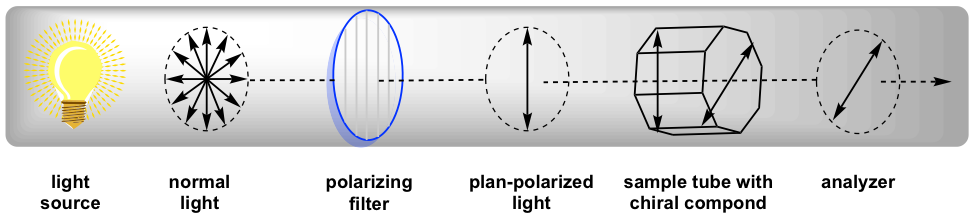
\includegraphics[width=.8\textwidth]{problems/figures/opticalRotationSchematic.png}
\end{center}

Nếu chiều dài của bình chứa dung dịch là \( L = 0.15 \, \text{m} \), góc xoay của phân cực ánh sáng là bao nhiêu, tức là tổng độ xoay quang học \( \Delta \theta \), tính bằng radian? Nhập đáp án dương nhỏ nhất cho câu hỏi này.
\end{problem}